%%%%%%%%%%%%%%%%%%%%%%%%%%%%%%%%%%%%%%%%%%%%%%%%%%%%%%%%%%%%%
%% Begin exercise %%
%%%%%%%%%%%%%%%%%%%%%%%%%%%%%%%%%%%%%%%%%%%%%%%%%%%%%%%%%%%%%

\ex{Flyback converter /}

%%%%%%%%%%%%%%%%%%%%%%%%%%%%%%%%%%%%%%%%%%%%%%%%%%%%%%%%%%%%%
%% Task 1: Flyback converter %%
%%%%%%%%%%%%%%%%%%%%%%%%%%%%%%%%%%%%%%%%%%%%%%%%%%%%%%%%%%%%%
\task{Flyback converter}
A flyback converter with an input voltage range $U_\mathrm{1} = \SI{300}{\volt} \, \dots \, \SI{900}{\volt}$ is used to supply the control electronics of a frequency inverter. The converter delivers a rated output power of  $P_\mathrm{2} = \SI{30}{\watt}$ at a regulated (constant) output voltage of  $U_\mathrm{2} = \SI{15}{\volt}$. The flyback converter is operated in discontinuous current mode with a constant frequency of  $f_\mathrm{p} = \SI{500}{\kilo\hertz}$. The transformation ratio of the transformer is $N_\mathrm{1}/N_\mathrm{2}=60/12$, the inductance of the primary winding is $L_\mathrm{1} = \SI{760}{\micro\henry}$. The coupling between the primary and secondary windings is ideal. You can assume stationary operation for all calculations.

%%%%%%%%%%%%%%%%%%%%%%%%%%%%%%%%%%%%%%%%%%%%%%%%%%%%%%%%%%%%%%%%%%%%%%%
 % Flyback converter Schematic
%%%%%%%%%%%%%%%%%%%%%%%%%%%%%%%%%%%%%%%%%%%%%%%%%%%%%%%%%%%%%%%%%%%%%%%
           
           \begin{figure}[htb]
                \begin{center}
                    \begin{circuitikz}[european currents,european resistors,american inductors]
                    \draw (0.5,0) to [short] ++(0.5,0)
                    to [diode, l=$D$]  ++(1.0,0)
                    to [short, -o, i=$i_2(t)$] ++(1.0,0)
                    to [open, o-o, v = $\hspace{2cm}u_2(t)$, voltage = straight] ++(0,-2) coordinate (A)
                    (-0.5,0) to [short, -o, i_<=$i_1(t)$] ++(-1.5,0)
                    to [open, o-o, v_= $u_1(t)\hspace{0.75cm}$, voltage = straight] ++(0,-3.75) coordinate (B)
                    (-0.5,0) to [inductor, n=l1] ++(0,-2) 
                    to [Tnpn, n=npn1, mirror] ++(0,-1.75) coordinate (C)
                    (0.5,0) to [inductor, n=l2, mirror] ++(0,-2) coordinate (D)
                    (D) to [short, -o] (A)
                    (C) to [short, -o] (B);
                    \draw let \p1 = (npn1.B) in node[anchor=south] at (\x1,\y1) {$T$};
                    \path (l1.ul dot) node[circ]{}
                        (l2.ur dot) node[circ]{};
                    \draw (l1.midtap) node[left]{$N_1$}
                    (l2.midtap) node[right]{$N_2$};
                    \draw[double, double distance=3pt, thick] let \p1=(l1.core west), \p2=(l2.core east) in (\x1/2+\x2/2, \y1) -- (\x1/2+\x2/2, \y2);
                \end{circuitikz}
            \end{center}
                \caption{Flyback converter topology}
                \label{fig:flyback_converter_topology}
            \end{figure}
        

\begin{table}[ht]
    \centering  % Zentriert die Tabelle
    \begin{tabular}{llll}
        \toprule
        
        Input voltage: &  $U_{\mathrm{1}} = \SI{300}{\volt} \, \dots \, \SI{900}{\volt}$ & Output voltage: & $U_{\mathrm{2}} = \SI{15}{\volt}$ \\ 
        Output power: & $P_2 = \SI{30}{\watt}$  & Transformation ratio: & $N_\mathrm{1}/N_\mathrm{2}=60/12$ \\ 
        Inductance of the primary winding: & $L_\mathrm{1} = \SI{760}{\micro\henry}$ & Switching frequency: & $f_{\mathrm{s}} = \SI{50}{\kilo\hertz}$ \\ 
        \bottomrule
    \end{tabular}
    \caption{Parameters of the boost converter.}  % Beschriftung der Tabelle
    \label{table:ex04_Parameters of the circuit}
\end{table}

\subtask{The input voltage is $U_\mathrm{1}=\SI{760}{\volt}$ at rated power at the output. What is the peak value $\hat I_\mathrm{1}$ of the primary current $i_\mathrm{1}$? What is the peak value $\hat I_\mathrm{2}$ of the secundary current $i_\mathrm{2}$? Calculate the duty cycle of the transistor for this operating case.}

\begin{solutionblock}
\begin{equation}
    P_\mathrm{2} = W_\mathrm{L} f_\mathrm{p}
\end{equation}

\begin{equation}
    W_\mathrm{L} = \frac{1}{2}L_\mathrm{1}\hat I_\mathrm{1}^2 
\end{equation}

\begin{equation}
    \hat I_\mathrm{1} = \sqrt{\frac{2P_\mathrm{2}}{L_\mathrm{1}f_\mathrm{p}}}= \sqrt{\frac{2\cdot\SI{30}{\watt}}{\SI{760}{\micro\henry}\cdot\SI{50}{\kilo\hertz}}}=\SI{1.257}{\ampere}
\end{equation}

\begin{equation}
    \hat I_\mathrm{1} = \hat I_\mathrm{2}
\end{equation}

\begin{equation}
    \hat I_\mathrm{2} = \hat I_\mathrm{1} \frac{N_\mathrm{1}}{N_\mathrm{2}} = \SI{1.257}{\ampere} \cdot \frac{60}{12} = \SI{6.28}{\ampere}
\end{equation}
Because of CCM the duty cycle $D$ is expressed .....
\begin{equation}
    \frac{U_2}{U_1} = \frac{D^2}{2} \frac{\Delta i_\mathrm{m,max}}{\overline{i}_2} \label{eq:Duty cycle ex04}
\end{equation}
Because of the unknown $\Delta i_\mathrm{m,max}$ this value has to be calculate first as
\begin{equation}
    \Delta i_\mathrm{m,max}= \frac{T_\mathrm{s} \cdot U_1}{L} = \frac{\frac{1}{\SI{50}{\kilo\hertz}}\cdot \SI{760}{\volt}}{\SI{760}{\micro\henry}}=\SI{20}{\ampere}.
\end{equation}
Now $\Delta i_\mathrm{m,max}=\SI{20}{\ampere}$ can be used in \eqref{eq:Duty cycle ex04}:

\begin{equation}
    D = \sqrt{\frac{2U_2\overline{i}_2}{U_1\Delta i_\mathrm{m,max}}} = \sqrt{\frac{2\cdot \SI{15}{\volt}\cdot\SI{30}{\watt}}{\SI{760}{\volt}\cdot\SI{15}{\volt}\cdot\SI{20}{\ampere}}} = 0.063.
\end{equation}

\end{solutionblock}

\subtask{The input voltage is  $U_\mathrm{1}=\SI{382}{\volt}$ at nominal load. Calculate and sketch the following voltage and current curves for this operating case over one cycle period: $u_\mathrm{T}(t), u_\mathrm{s}(t), i_\mathrm{2}(t), i_\mathrm{1}(t)$ (Note: corresponds to the switch-on time of the transistor).}

\begin{solutionfigure}[htb]
    \centering
    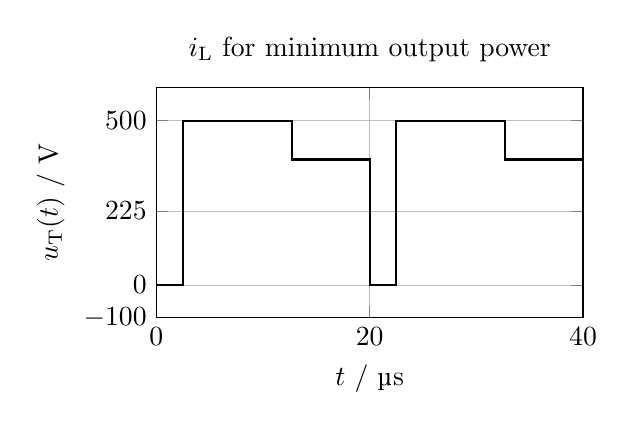
\begin{tikzpicture}
    \begin{axis}[
        width=7cm, height=4.5cm,
        grid=both,
        major grid style={line width=.2pt,draw=gray!50},
        minor grid style={line width=.1pt,draw=gray!20},
        xlabel={$t$ / µs},
        ylabel={$u_\mathrm{T}(t)$ / V},
        title={$i_\mathrm{L}$ for minimum output power},
        xmin=0, xmax=40,
        ymin=-100, ymax=600,
        xtick={0, 20, 40},
        ytick={-100, 0, 225, 500},
        ]
        % Einschaltverhalten graph
        \addplot[
            thick,
            mark=none,
            color=black,
        ] coordinates {
            (0,0) (2.5,0) (2.5, 500) (12.7, 500) (12.7, 382) (20, 382) (20, 0) (22.5, 0)(22.5, 500) (32.7, 500) (32.7, 382) (40, 382)
        };
    \end{axis}
    \end{tikzpicture} 
    \hspace{1cm} % Abstand zwischen den beiden Diagrammen
    \caption{Display of the voltage $u_\mathrm{T}(t)$.}
    \label{fig:voltageTransistorPeriodTask1}
    \end{solutionfigure}
    


\subtask{The input voltage is  $U_\mathrm{1}=\SI{382}{\volt}$ at nominal load. Determine the mean value $\overline i_\mathrm{T}$ and the effective value of the current $i_\mathrm{T, rms}$ through the transistor. Determine the mean value $\overline i_\mathrm{D}$ and the effective value of the current $i_\mathrm{D, rms}$ through the diode. What is the maximum reverse voltage load $u_\mathrm{T, max}$ of the transistor? What is the maximum reverse voltage load $u_\mathrm{D, max}$ of the diode? Calculate the fluctuation range $\Delta i_\mathrm{C, pp}$ of the current $i_\mathrm{C}$ in the output capacitor.}

\subtask{The input voltage is  $U_\mathrm{1}=\SI{382}{\volt}$ at nominal load.How much energy is transferred from the input to the output per switching period $\Delta E$ and what is the resulting average power? What happens if there is no ideal voltage source on the output side but an unloaded capacitor and the circuit is operated with $D>0$?}